\newcommand{\indentar}[1][1em]{\mbox{\hspace{#1}}}
\newcommand{\signo}[2][©]{
  \begingroup
  \noindent\makebox[1em][l]{#1}%
  \hangindent=1em\hangafter=1
  #2\par
  \endgroup
}
\thispagestyle{empty}

\mbox{\nobreakspace}

\vfill

\begin{minipage}[t]{4.46in}
  \fontsize{7pt}{8pt}\selectfont

  \begin{center}
    \includegraphics[width=4cm]{esIcons/logos.pdf}
  \end{center}

  \vspace{0.8cm}

  \begin{minipage}[t]{0.45\textwidth}
    \begin{raggedright}
      \signo{Universidad Distrital Francisco José de Caldas}
      \signo{Facultad de Ingeniería}
      \signo{\loauthors\ (autores)}

      \vspace{1.2em}

      \textopb{ISBN:} 978-958-787-951-3\\
      \textopb{ISBN digital:} 978-958-787-952-0\\
      \textopb{ISBN ePub:} 978-958-787-953-7

      \vspace{1.2em}

      \textopb{DOI:} \href{https://doi.org/10.69740/UD.9789587879513.9789587879537}{\mbox{https://}\nolinkurl{doi.org/10.69740/UD.9789587879513.9789587879537}}

      \vspace{1.2em}

      Primera edición, abril de 2026

      \vspace{1.2em}

      \textopb{Gestión editorial}\\
      \indentar Editorial UD

      \vspace{0.5em}

      \textopb{Corrección de estilo}\\
      \indentar Hipertexto SAS

      \vspace{0.5em}

      \textopb{Diagramación}\\
      \indentar Hipertexto SAS

      \vspace{0.5em}

      \textopb{Diseño de cubierta}\\
      \indentar Editorial UD
    \end{raggedright}
  \end{minipage}\hfill
  \begin{minipage}[t]{0.49\textwidth}
    \begin{raggedright}
      \textopb{Editorial UD}

      Universidad Distrital Francisco José de Caldas\\
      Carrera 24 n.º 34-37 Bogotá, D. C., Colombia\\
      Teléfono: 6013239300 ext. 6202\\
      Correo electrónico: \href{mailto:publicaciones@udistrital.edu.co}{publicaciones@udistrital.edu.co}

      \vspace{1.2em}

      \begingroup\fontsize{6pt}{7pt}\opseries\selectfont
      \textopb{Cláusula de responsabilidad:}

      Editorial UD no es responsable de las opiniones y de la
      información recogidas en el presente texto. Los autores
      asumen de manera exclusiva y plena toda responsabilidad
      sobre su contenido, ya sea este propio o de terceros,
      declarando en este último supuesto que cuentan con
      la debida autorización de terceros para su publicación.
      Igualmente, expresan que no existe conflicto de interés
      alguno en relación con los resultados de la investigación
      propiedad de tales terceros. En consecuencia, los autores
      serán responsables civil, administrativa o penalmente, frente
      a cualquier reclamo o demanda por parte de terceros,
      relativa a los derechos de autor u otros derechos que se
      vulneren como resultado de su contribución.

      \vspace{1.2em}

      \textopb{Todos los derechos reservados.}

      Esta obra no puede ser reproducida sin el permiso previo
      escrito de la Unidad de Publicaciones de la Universidad
      Distrital Francisco José de Caldas.

      Hecho en Colombia.
      \endgroup
    \end{raggedright}
  \end{minipage}

  \vspace{0.8cm}

  \newsavebox{\catalografica}

  \begin{lrbox}{\catalografica}
    \begin{minipage}[t]{\textwidth}
      \fontsize{7pt}{8pt}\opseries\selectfont
      \begin{center}
        \textit{Sistema de Bibliotecas de la Universidad Distrital Francisco José de Caldas}\\
        \textit{Catalogación en la publicación (CEP)}
      \end{center}

      \vspace{0.6em}

      \begin{raggedright}
        \indentar[3em] Ingeniería ambiental: saneamiento ambiental en establecimientos / Yenny Tatiana Romero
        Ladino ... [y otros 3 autores]. -- Primera edición. -- Bogotá : Universidad Distrital Francisco José de
        Caldas, 2023. 91 páginas ; 24 cm. (Colección tierra y vida)

        \vspace{0.6em}

        ISBN: 978-958-787-528-7 \quad
        ISBN digital: 978-958- 987-530-0 \quad
        ISBN ePub: 978-958-787-529-4

        \vspace{0.6em}

        \indentar[3em] 1.~Saneamiento ambiental -- Mediciones 2.~Auditoria ambiental 3.~Ingeniería ambiental
        4.~Salud pública.\enspace I.~Romero Ladino, Yenny Tatiana, autora II.~Peñaranda Galvis, Vidal Fernando, autor
        III.~Rodríguez Miranda, Juan Pablo, autor IV.~Sánchez Céspedes, Juan Manuel, autor V.~Serie

        \vspace{0.6em}

        \indentar[3em] 628.51: CDD 21 edición.
      \end{raggedright}
    \end{minipage}
  \end{lrbox}

  \begin{center}
    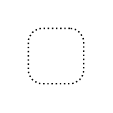
\begin{tikzpicture}
      \node[draw,
        rounded corners=0.5em,
        densely dotted,
        line width=0.5pt,
        inner xsep=1em,
      inner ysep=1em]
      {\usebox{\catalografica}};
    \end{tikzpicture}
  \end{center}
\end{minipage}

\newpage
